\documentclass[class=article , crop=false, titlepage, twoside, multi={itemize, figure, verbatim}, float=false]{standalone}

\usepackage{import} % Required for importing other .tex docs.  (import uses everything bw Begin and End Doc)
\usepackage{float} % Required for specifying the exact location of a figure or table
\usepackage{graphicx} % Required for including images
\usepackage{wrapfig}
\usepackage[pdftex,breaklinks,colorlinks=true,linkcolor=black,citecolor=blue,urlcolor=red,linktocpage=false,pagebackref=true,filecolor=magenta]{hyperref}%http://www.tug.org/applications/hyperref/manual.html#x1-100003.6
\usepackage{cite}
\usepackage[toc,title,page]{appendix}
\usepackage{pdfpages} % enables loading a pdf into the doc
\usepackage{makeidx}
\usepackage{glossaries} % must be after hyperref
\usepackage{blindtext}
\usepackage{enumitem}
%\usepackage{caption}

%\setlist[description]{leftmargin=\parindent,labelindent=\parindent}

%\renewcommand*{\bibname}{References} % renames the bibliography

\newcommand{\HRule}{\rule{\linewidth}{0.5mm}} % Command to make the lines in the title page

\graphicspath{{img/}{GIS_ChampionSection/img/}{awardsChapter/GIS_ChampionSection/img/}{brandPart/awardsChapter/GIS_ChampionSection/img/}{img/}{pairedProgSection/img/}{methodChapter/pairedProgSection/img/}{methodPart/methodChapter/pairedProgSection/img/}{documentationSection/img/}{methodChapter/documentationSection/img/}{methodPart/methodChapter/documentationSection/img/}{docStorageOrgSection/img/}{methodChapter/docStorageOrgSection/img/}{methodPart/methodChapter/docStorageOrgSection/img/}{QGisSection/img/}{toolsChapter/QGisSection/img/}{servicePart/toolsChapter/QGisSection/img/}{ESRISection/img/}{toolChapter/ESRISection/img/}{servicePart/toolChapter/ESRISection/img/}{../../../../source/}{../../source/}{servicePart/applicationsChapter/treasurerSection/img/}}

%\setlength\parindent{0pt} % eliminates indents


\def\titlename{Batch PDF Optimization\\ \medskip\large with Python, batch files, and ghostscript}

\title{\HRule % Horizontal Line added
\\[.4cm] % space
\begin{figure}[H] % included image
\begin{center}	% centered horizontally
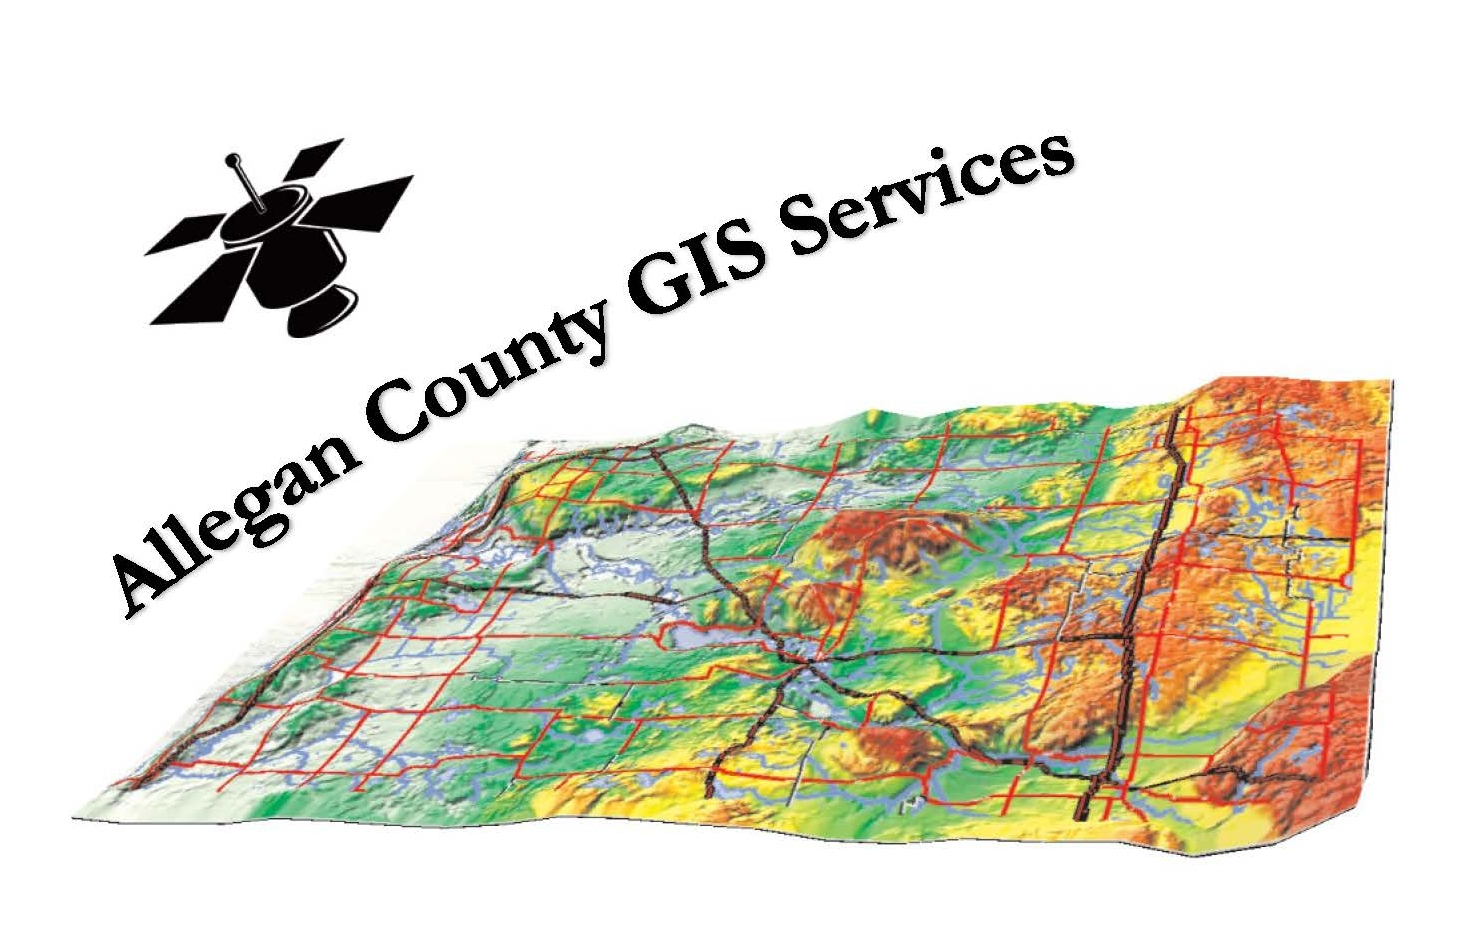
\includegraphics[scale=.45]{GIS_Logo_better.jpg}
\end{center}
\end{figure}
\Huge \bfseries \titlename \\ % Title text
\HRule \\[.4cm] % Horizontal Line added
\author{\Large Allegan County GIS \\\Large www.allegancounty.org/gis} % defines author
}  % inputs common title

\begin{document}% document begins

\ifstandalone
\maketitle % creates title page
\clearpage
\tableofcontents % creates TOC
\clearpage
\fi

\clearpage

\subsection{PDF Optimizer}
\subsubsection{Pupose and Summary}
\textbf{Workflow Purpose:} Optimization of a large number of pdf docs.\\
\textbf{Workflow Summary:} Uses Python to create a list of .pdf docs in a folder and creates a batch file to optimize the pdfs in the list to another location.  The batch process calls ghost script for the optimization.

\subsubsection{requirements}
Opensource software:
\begin{itemize}
\item ghostscript
\item python 2.7 and a Python IDE
\item A text editor
\end{itemize}
paragraph{Python(2.7)}

\paragraph*{Note:} The output of this script is bdoc.txt, Save as a .bat to execute the optimize.

\paragraph*{Script that creates a batch file}
\begin{verbatim}
import os, sys

project = os.path.dirname(os.path.dirname(__file__))
processing = os.path.join(project, 'processing')
#source = os.path.join(project,'source')
build = os.path.join(project,'build')
sourcepdf = os.path.join(build, '20180716')

inString1 = "gswin32 -sDEVICE=pdfwrite -dCompatibilityLevel=1.4
-dPDFSETTINGS=/ebook -dNOPAUSE -dQUIET -dBATCH
-sOutputFile=J:\\Projects\\2018ParcelAtlas\\build\\optimized\\"

inString2 = " J:\\Projects\\2018ParcelAtlas\\build\\20180716\\"

batchdoc = os.path.join(processing,"bDoc.txt")

#   Main
################################################################################

if __name__ == "__main__":

    list1 = os.listdir(sourcepdf)
    l = open(batchdoc,'w')
    for i in list1:
        newi = i[1:]
        print newi
        t = inString1 + newi + inString2 + i + "\n"
        print t
        l.write(t)

    l.close()

\end{verbatim}

\subsubsection{ghostscript}

\paragraph{About}
ghostscript is used for the optimization. ghostscript is an interpreter for the PostScript language and for PDF~\cite{ghostscript1}.
\paragraph{Licensing}
ghostscript is available opensource under AGPL conditions.  more information can be found \href{https://www.ghostscript.com/license.html}{here}.
\paragraph{Download}
ghostscript can be downloladed \href{https://www.ghostscript.com/download/gsdnld.html}{here}.


\subsubsection{Windows batch files}
A line from the batch file looks like:\\
\begin{verbatim}



gswin32 -sDEVICE=pdfwrite -dCompatibilityLevel=1.4
 -dPDFSETTINGS=/ebook -dNOPAUSE -dQUIET -dBATCH
 -sOutputFile=J:\Project\2018ParcelAtlas\build\optimized\
 02-001-001-00.pdf J:\Projects\2018ParcelAtlas\build\20180716
 \_02-001-001-00.pdf

\end{verbatim}

\end{document}
